\documentclass[12pt,Bold,letterpaper,TexShade]{mcgilletdclass}
%\usepackage[dvips,final]{graphicx}
\usepackage[dvips]{geometry}
\usepackage{texshade}

% Questions to ask when contacting McGill regarding thesis format
% 0) Possible not to use the mcgilletdclass? And if not, what must not be changed as per 'Please note that required commands must not be changed if your thesis is to be correctly converted to XML for the McGill EThesis Project.'?
% 1) Links in TOC to Dedication through Abstracts and Appendices do not go to the proper page. How to fix this?
% 2) Ugly and inconsistent font for "TOC"s and "References". How to fix this without having the boldface appear in the main TOC?
% 3) Why might it be necessary to modify some of the commands defined in the documentclass?


% NOTES:
% To get bibtex to work correctly, perform the following steps:
% 1) In the command prompt, type 'pdflatex mydoc.tex'
% 2)                        type 'bibtex mydoc'
% 3)                        type 'pdflatex mydoc.tex'
% If there were no errors, the bibliography and references should now be displayed.
% http://tex.stackexchange.com/questions/85147/mac-os-latex-install-not-compiling-bibliography

%%%%%%%%%%%%%%%%%%%%%%%%%%%%%%%%%%%%%%%%%%%%%%%%%%%%%
% My packages

\usepackage[usenames,dvipsnames]{xcolor}
\usepackage{wrapfig}
\usepackage{lettrine}
\usepackage{amssymb}
\usepackage{mdwlist}
\usepackage{color}
\usepackage{capt-of}
\usepackage{multirow}
\usepackage{graphicx}
\usepackage{epsfig}
\usepackage[euler]{textgreek}
\usepackage{epstopdf}
\usepackage{mathtools}
\usepackage{amsmath,amsthm,mathtools}
\usepackage{relsize}
\usepackage{breqn}
\usepackage{standalone}
\usepackage{tikz}
\usepackage{lineno}
\usepackage{textcomp}
\numberwithin{equation}{section}

\newlength\tindent
\setlength{\tindent}{\parindent}
\setlength{\parindent}{0pt}
\renewcommand{\indent}{\hspace*{\tindent}}

% For Theorems, Lemmas, Proofs, etc; 
% http://www.maths.tcd.ie/~dwilkins/LaTeXPrimer/Theorems.html
\newtheorem{theorem}{Theorem}[section]
\newtheorem{lemma}[theorem]{Lemma}
\newtheorem{proposition}[theorem]{Proposition}
\newtheorem{corollary}[theorem]{Corollary}

\usepackage{caption}
\usepackage{subcaption}
\usepackage{soul}
\usepackage{cases}

\usepackage{hyperref}
\hypersetup{
    colorlinks,
    citecolor=blue,
    filecolor=black,
    linkcolor=blue,
    urlcolor=black,
}
\usepackage{appendix}
\usepackage{color}

% For section symbol
\def\Snospace~{\S{}}
\renewcommand*\sectionautorefname{\Snospace}
\renewcommand*\subsectionautorefname{\Snospace}
\renewcommand*\subsubsectionautorefname{\Snospace}

\newcommand{\slfrac}[2]{\left.#1\middle/#2\right.}
\newcommand{\cmark}{\ding{51}}%
\newcommand{\xmark}{\ding{55}}

% Define commands to assure consistent treatment throughout document
\newcommand{\eqnref}[1]{(\ref{#1})}
\newcommand{\class}[1]{\texttt{#1}}
\newcommand{\package}[1]{\texttt{#1}}
\newcommand{\file}[1]{\texttt{#1}}
\newcommand{\BibTeX}{\textsc{Bib}\TeX}

\usepackage{titling}
\usepackage[parfill]{parskip}
\usepackage{bm}

\newcommand{\mat}[1]{\bm{{#1}}}
\newcommand{\vect}[1]{\bm{{#1}}}
%\newcommand{\mat}[1]{\underline{\overline{{#1}}}}
%\newcommand{\vect}[1]{\underline{{#1}}}

\newcommand{\coloneqqspace}{\coloneqq \hspace{1mm}}

\allowdisplaybreaks[1]

\expandafter\def\expandafter\normalsize\expandafter{%
    \normalsize
    \setlength\abovedisplayskip{3pt}
    \setlength\belowdisplayskip{3pt}
    \setlength\abovedisplayshortskip{3pt}
    \setlength\belowdisplayshortskip{3pt}
}

\raggedbottom



\usepackage[T1]{fontenc}

\usepackage[breakable,theorems,skins]{tcolorbox}
\tcbset{enhanced}

\DeclareRobustCommand{\highlightbox}[2][gray!20]{%
\begin{tcolorbox}[   %% Adjust the following parameters at will.
        breakable,
        left=0pt,
        right=0pt,
        top=0pt,
        bottom=0pt,
        colback=#1,
        colframe=#1,
        width=\dimexpr\textwidth\relax, 
        enlarge left by=0mm,
        boxsep=5pt,
        arc=0pt,outer arc=0pt,
        ]
        #2
\end{tcolorbox}
}
% http://tex.stackexchange.com/questions/46828/how-to-highlight-important-parts-with-a-gray-background



%%%%%%%%%%%%%%%%%%%%%%%%%%%%%%%%%%%%%%%%%%%%%%%%%%%%%

%%% McGill Guidelines
% It is suggested that the \paragraph command be used for third-level subheadings.
% Captions must be placed above tables and below figures. \TableCaption{text} is for tables and \FigureCaption{text} is for figures.
% \TableCaptionOpt{text1}{text2} is another command for the similar use. Here, text1 will appear in the list of tables; text2 is the actual caption of a table. Similarly, \FigureCaptionOpt{text1}{text2} is for figures.

%%%%%%%%%%%%%%%%%%%%%%%%%%%%%%%%%%%%%%%%%%%%%%%%%%%%%
%% Have you configured your TeX system for proper  %%
%% page alignment? See the McGillETD documentation %%
%% for two methods that can be used to control     %%
%% page alignment. One method is demonstrated      %%
%% below. See documentation and the ufalign.tex    %%
%% file for instructions on how to adjust these    %%
%% parameters.                                     %%
\addtolength{\hoffset}{0pt}                        %%
\addtolength{\voffset}{0pt}                        %%
%%                                                 %%
%%%%%%%%%%%%%%%%%%%%%%%%%%%%%%%%%%%%%%%%%%%%%%%%%%%%%

%%%       Define student-specific info
% Note: All caps in title.
%\SetTitle{\huge{Target-Based Adaptation Using the\\Discontinuous Petrov-Galerkin Method}}%
%\SetAuthor{Philip Zwanenburg}%
%\SetDegreeType{Bachelor of Engineering}%
%\SetDepartment{Department of Mechanical Engineering}%
%\SetUniversity{McGill University}%
%\SetUniversityAddr{Montreal,Quebec}%
%\SetThesisDate{2018-08-31}%
%\SetRequirements{A thesis submitted to\\McGill University\\in partial fulfillment of the requirements of the degree of\\Doctor of Philosophy}%
%\SetCopyright{\textcopyright\hspace{1mm}Philip Zwanenburg, 2018}%

%%\usepackage[nottoc]{tocbibind} % Don't include ToC line in ToC
%
%\usepackage{tocloft}
%%\renewcommand\contentsname{Table of Contents}
%\renewcommand\cfttoctitlefont{\hfil\mdseries} % use "\bfseries" if you want it in bold
%\renewcommand{\cftaftertoctitle}{\hfil}
%\renewcommand{\cftchapfont}{\mdseries}
%\renewcommand{\cftchappagefont}{\mdseries}
%\renewcommand{\cftchapleader}{\cftdotfill{\cftdotsep}}

\begin{document}

\begin{titlepage}
    \centering
    \large
    {\huge TARGET-BASED ADAPTATION USING \\ THE DISCONTINUOUS \\ \vspace{4mm} PETROV-GALERKIN METHOD}
    \vfill
    {\Large Philip Zwanenburg}\\
    Bachelor of Engineering\\
    \vfill
    Department of Mechanical Engineering\\
    McGill University\\
    Montreal, Quebec\\
    \vfill
    \date{\today}
    \vfill
    A thesis submitted to\\McGill University\\in partial fulfillment of the requirements of the degree of\\Doctor of Philosophy\\
    \vfill
    
\includegraphics[width=0.2\textwidth]{./figures/McGillcrest.eps}
    \vfill
    {\normalsize \textcopyright\hspace{1mm}Philip Zwanenburg, \the\year}\\
    \vfill
    \vfill
\end{titlepage}

%\maketitle

\begin{romanPagenumber}{2}%

\SetDedicationName{\uppercase{Dedication}}%
\SetDedicationText{This thesis is dedicated to those who have fuelled my interest in numerical analysis through their genious, creativity and passion. {\color{red} Include best graphic or logo}}%
\Dedication%

\SetAcknowledgeName{\uppercase{Acknowledgements}}%
\SetAcknowledgeText{
{\color{red}ToBeDone}\\
Don't forget NSERC+McGill Funding
}%
\Acknowledge%


%%%%%%%%%%%%%%%%%%%%%%%%%%%%%%%%%%%%%%%%%%%%%%%%%%%%%
%%         English Abstract                        %%
%%%%%%%%%%%%%%%%%%%%%%%%%%%%%%%%%%%%%%%%%%%%%%%%%%%%%
\SetAbstractEnName{\uppercase{Abstract}}%
\SetAbstractEnText{
{\color{red}ToBeDone}
}
\AbstractEn%

%%%%%%%%%%%%%%%%%%%%%%%%%%%%%%%%%%%%%%%%%%%%%%%%%%%%%
%%         French Abstract                         %%
%%%%%%%%%%%%%%%%%%%%%%%%%%%%%%%%%%%%%%%%%%%%%%%%%%%%%
\SetAbstractFrName{\uppercase{ABR\'{E}G\'{E}}}%
\SetAbstractFrText{
{\color{red}ToBeDone}
}%
\AbstractFr%

\begingroup
\hypersetup{linkcolor=black}
\TOCHeading{\uppercase{Table of Contents}}%
\LOTHeading{\uppercase{List of Tables}}%
\LOFHeading{\uppercase{List of Figures}}%
\tableofcontents %
\listoftables %
\listoffigures %
\endgroup

\end{romanPagenumber}

%\mainmatter %
 
%%%%%%%%%%%%%%%%%%%%%%%%%%%%%%%%%%%%%%%%%%%%%%%%%%%%%%%%%%%%%%%%%%
\chapter{Introduction}
%%%%%%%%%%%%%%%%%%%%%%%%%%%%%%%%%%%%%%%%%%%%%%%%%%%%%%%%%%%%%%%%%%
\section{Motivation \& Open Topics}

The use of computational fluid dynamics (CFD) tools for the numerical analysis of fluid flows has significantly reduced costs associated with aerodynamic design over the past several decades. As computing systems have become increasingly powerful, there has been a corresponding advance in the equations employed for flow simulation (initially beginning with potential equations and now using the full Navier-Stokes equations) as well as in the resolution of complex flow phenomena.

Finite volume methods currently represent the industry and, to a great extent, academic standard for the solution of partial differential equations (PDEs) in the aerospace community. This is in large part due to their robustness in the presence of steep gradients in the flow as well as their ability to model geometrically complex objects as a result of the possibly unstructured nature of the volumes. However, finite volume schemes are inherently second order accurate, making their usage inefficient when flow solutions are smooth. In these cases, it is advantageous to use higher-order functions for the representation of the solution, resulting in solution convergence at greater rates than second order as well as necessitating fewer degrees of freedom (DOF) to obtain similar levels of solution resolution. One would thus like to employ spectral methods because of their exponential convergence properties, however these methods are unsuitable in the presence of complex geometry. Pseudo-spectral methods (which can be thought of as a spectral method being used within each control volume of a finite volume scheme) have become the most popular choice when attempting to address the concern of employing high-order accurate (greater than second order) solution representation in the presence of complex geometry. 

The discontinuous Galerkin (DG) method, initially proposed by Reed et al.~\cite{reed1973} and subsequently analyzed for the solution of systems of conservation laws~\cite{cockburn1991,cockburn1989a,cockburn1989b,cockburn1990,cockburn1998}, has become the most popular choice of high-order scheme in the CFD community.  Despite its widespread usage, there are still several major issues related to the standard DG method:

\begin{itemize}
\item High computational complexity with increasing order of accuracy;
\item Restrictive Courant-Friedrichs-Lewy (CFL) conditions for explicit time stepping and suboptimal dissipation and dispersion characteristics for wave propagation;
\item Difficulty in generating meshes for complex geometrical objects as well as in converting low-order meshes provided by standard mesh generators to high-order meshes;
\item Improper test space for best approximation in the energy norm when applied to hyperbolic PDEs. %Niemi2012
\end{itemize}

The last of these issues provides the motivation for the thesis, however, many difficulties arising from the other listed problems have already been encountered simply while setting up the framework to begin the novel research. With particular regard to the representation of complex curved geometry, it has been observed that improper geometry treatment can contribute significant error to a flow simulation, potentially eliminating any advantages obtained from the use of better test spaces, for example.

%%%%%%%%%%%%%%%%%%%%%%%%%%%%%%%%%%%%%%%%%%%%%%%%%%%%%%%%%%%%%%%%%%
\subsection{Computational Complexity}
\label{sec:Comp_comp}
{\color{red} Provide links to sections where related results are provided if available}

Significant progress has been made with regard to the improvement of the DG method's computational complexity, notably through the exploitation of sum factorization techniques, originally proposed by Orszag~\cite{orszag1980} and now employed in the tensor-product Spectral element method (SEM) of Kopriva~\cite{kopriva2009} and for general elements using collapsed tensor-product spaces by Karniadakis et al.~\cite{karniadakis1999}. When explicit methods are used, use of the sum factorization technique reduces the growth in computational complexity from $O(N^{2d})$ to $O(N^{d+1})$ where $d$ is the dimension of the problem and $N = P+1$ where $P$ is the order of the method. Savings for implicit schemes are even greater and further, the appropriate decomposition of element bases into corner, edge, facet, and volume modes allows for the ability to statically condense out the volume modes, significantly reducing the growth rate of globally coupled DOF as the order of the solution is increased in global matrix inversion stages. Sum factorization ideas have traditionally mainly been used for relatively high solution polynomial orders ($P \geq 8$) {\color{red} (reference for this, maybe sherwin)} due to the lack of improvement over standard operators at lower orders, a minor goal of this work was to demonstrate that the algorithm is also relevant in the polynomial range considered here ($0 \leq P \leq 4$). {\color{red} Refer to section confirming the break even point. Compare with sparse standard (collocated), discuss cost of application of inverse mass matrix (uncollocated), discuss cost of linear solve (implicit, uncollocated).}

Another technique pursued for computational complexity minimization is the use of collocated schemes. Collocated schemes, notably the nodal DG scheme~\cite{hesthaven2002,hesthaven2007}, minimize interpolation and integration costs by collocating solution and flux interpolation nodes with cubature nodes. While this culminates in satisfactory results for linear PDEs solved on straight-sided elements, the use of higher-order accurate cubature rules is advocated in curved elements or when solving nonlinear systems of equations, destroying the collocation property of the scheme. It has also been demonstrated that simplex element ``alpha-optimized'' nodes~\cite{warburton2006} associated with the nodal DG scheme, were unsuitable when solving nonlinear PDEs due to significant aliasing errors~\cite{witherden2014}. This in turn spurred research into the derivation of triangular and tetrahedral element nodes which possess good interpolation properties and have an associated cubature rule, recovering at least volume collocation; this has been pursued by several authors~\cite{witherden2014,williams2014b,shunn2012}. However, cubature rules associated with these nodes are weak in the sense that they can not even exactly integrate linear PDEs on linear elements when cast in the variational weak DG framework which might degrade their accuracy and high-order convergence properties; the conclusions of Bassi et al.~\cite{bassi2013} suggest that this occurs for tensor-product elements.

A final avenue which has been pursued for the minimization of computational cost associated with high-order methods is the use of pre-integrated DG schemes~\cite{atkins1996} or DG-type schemes cast in differential form, notably the Energy Stable Flux Reconstruction (ESFR) schemes introduced in~\autoref{sec:CFL_diss_disp}. In these versions of the DG scheme, integral operations associated with the weak formulation of the DG scheme are performed in a preprocessing stage, eliminating many of the cubature operations associated with the original scheme. It is shown in {\color{red} link to scheme derivation section} that the majority of operators can be pre-computed in this fashion for both weak and strong forms of DG-type schemes and that it would be naive not to do so.

%%%%%%%%%%%%%%%%%%%%%%%%%%%%%%%%%%%%%%%%%%%%%%%%%%%%%%%%%%%%%%%%%%
\subsection{Restrictive CFL Condition and Suboptimal Dissipation and Dispersion Properties}
\label{sec:CFL_diss_disp}

As there is some level of subcell resolution in high-order schemes, the maximum CFL number decreases with the order of approximation of the solution on a fixed mesh. This results in restrictive time step sizes when solving problems explicitly. The recently introduced Flux Reconstruction (FR) schemes, initially proposed for tensor-product elements~\cite{huynh2007} and subsequently generalized to simplex elements~\cite{wang2009}, were originally presented as a unifying framework for DG-type schemes where stable time step limits greatly in excess of the standard DG scheme were achieved. However, restrictions on the type of flux reconstruction allowable while maintaining linear stability of the various schemes proposed by Huynh~\cite{huynh2007} were initially unclear. Appropriate choices for energy stability resulted in the derivation of the ESFR schemes, energy stable for linear advection on tensor-product elements~\cite{vincent2011} and for advection-diffusion on tensor-product elements~\cite{castonguay2013}; the extension to simplex elements has also been made~\cite{castonguay2012,williams2013,williams2014a}.

Within the ESFR framework, with different schemes parametrized simply by two parameters $c$ and $k$ (which can be associated with a scaling of the highest mode of the numerical flux correction), investigations were performed to find the values of $c$ and $k$ achieving the maximum stable time steps for linear advection-diffusion problems. These values were denoted as $c_+$ and $k_+$, allowing for time steps approximately twice as large as in the original DG formulation while maintaining the optimal order of convergence~\cite{castonguay2013,castonguay2012,williams2013,williams2014a}. A similar analysis relating to filtering of the numerical flux in the standard DG formulation also demonstrated that the stable time step could be increased while maintaining the optimal order of convergence~\cite{chalmers2014}. More recent work has focused on optimizing within an ESFR framework to find optimal flux reconstruction operators for the minimization of dissipation and dispersion~\cite{asthana2014}. Interestingly, it was found that there existed an FR operator, not fitting within the ESFR framework, which had significantly improved performance as compared to the optimal ESFR operator for the minimization of dissipation and dispersion. While the authors were unable to conclude that this method was energy stable, the extension of the energy stability envelope may make this possible~\cite{vincent2015}.

As the formulation of the ESFR schemes is extremely similar to that of the original DG scheme, it was natural that comparisons between the two would be made and it was eventually determined that ESFR schemes could be interpreted as modally filtered DG schemes. This was initially demonstrated in 1D and for straight-sided tensor product extensions~\cite{allaneau2011} and subsequently generalized to straight-sided simplex elements~\cite{williams2014a}. A related investigation proving the equivalence of certain ESFR schemes with DG variants on both straight-sided and curved tensor-product elements was also performed~\cite{degrazia2014,mengaldo2015}. More recently, equivalence between all ESFR schemes and modally filtered DG schemes on curved tensor-product and simplex elements was demonstrated, with the important conclusion that ESFR schemes can be formulated as a weak DG scheme where discontinuous edge flux is substituted for numerical edge flux correction~\cite{zwanenburg2016}. Given the theoretical justifications for the numerical flux and the significant computational effort expended to compute it, this interpretation puts the modification of its contribution to the residual into question, despite increasing the stable time step size. It was further demonstrated that ESFR schemes are inherently less efficient than DG schemes in weak form when solving problems implicitly.

%%%%%%%%%%%%%%%%%%%%%%%%%%%%%%%%%%%%%%%%%%%%%%%%%%%%%%%%%%%%%%%%%%
\subsection{Treatment of Complex Geometry}

The proper treatment of complex geometry in high-order DG-type methods has been shown to be crucial. In the seminal work on the topic, it was demonstrated that curved geometry had to be represented in an isoparametric space of order $P$ for all solution polynomial orders $P \ge 2$ and in a superparametric space of second order in the case of first order solution representation in order to maintain the optimal convergence properties of these schemes, in two dimensions (2D)~\cite{bassi1997}. It was noted that low-order geometry representation results in deterioration of solution quality as the order of the scheme is increased, due to rarefaction waves being formed at vertices of polygonal mesh surfaces~\cite{krivodonova2006}. 

As the majority of mesh generators only provide linear meshes, a necessary inclusion in any high-order spectral element code is the projection of an initially straight-sided mesh to the curved geometry. This projection is commonly achieved through the use of transfinite blending function interpolation, first proposed by Gordon et al. for tensor-product elements~\cite{gordon1973} and subsequently generalized to simplex elements~\cite{nielson1979,haber1981,szabo1991,lacombe1988,dey1997,xie2013}. Assuming that corner nodes are located on the curved geometry, the process proceeds by sequentially projecting straight edge and facet nodes to the curved geometry followed by the application of a blending operation which appropriately displaces volume nodes (not touching the boundary). Ensuring that the error in the curved geometry representation converges at the same rate as the solution and the need for parametrization of arbitrary 3D curved surfaces represent two major challenges.

While errors due to improper geometry representation may only begin to manifest themselves at very fine levels of solution resolution, for high-order methods, these levels of accuracy are achievable. Further, if these geometric errors result in decreasing convergence rates of high-order methods, then the increase in the computational complexity would be incurred with no additional benefit, rendering these schemes useless. While optimal convergence orders for nonlinear hyperbolic cases have been demonstrated on curved geometry by many authors in 2D, the geometric complexity of the test cases used for these demonstrations has been minimal, generally with the possibility of employing analytic surface parametrization or using $C^{\infty}$ boundary functions. Curved surface representation is most commonly achieved using nodal geometry interpolation through a set of surface geometry nodes obtained from an arc length surface parametrization. To the author's knowledge, optimal convergence orders have never been published for any 3D simulation of nonlinear hyperbolic systems of equations over curved geometry. In 3D, additional geometric concerns must also be taken into account such as the enforcement of certain metric identities in order to ensure ``free-stream preservation" (i.e. avoid violations of conservation resulting only from curved geometry treatment)~\cite{kopriva2006}.

It is important to note that the discussion above assumed that a valid linear mesh could initially be generated for the complex geometry to be modelled in the simulation. In fact, it has recently been estimated that approximately 80\% of overall analysis time in the aerospace industry, among others, is devoted to (linear) mesh generation~\cite{hughes2005}, resulting in serious challenges when attempting to interface between simulated aerodynamic shape optimized profiles and the Computer Aided Design (CAD) model, for example. This motivated the formulation of isogeometric analysis where the solution is represented using the same basis as the CAD geometry, allowing for perfect geometric representation at any level of mesh refinement and seamless interfacing with CAD modelling~\cite{hughes2005}. The competitiveness of this new approach with existing methods has already been demonstrated in numerous benchmark test cases in both structural and fluid mechanics. The Non-uniform rational basis spline (NURBS) enhanced finite element method (NEFEM) in which the standard DG method is employed in the majority of the solution domain while isogeometric analysis is employed in curved elements has also recently been shown to provide superior results to standard DG discretizations on all test cases considered~\cite{sevilla2008,sevilla2011}. A further significant advantage of isogeometric analysis is that no interfacing with the CAD geometry would be required while performing mesh optimization during scheme execution, making these optimization algorithms suitable for the simulation of flow over vastly more complex geometric objects than those generally used for academic purposes.

%%%%%%%%%%%%%%%%%%%%%%%%%%%%%%%%%%%%%%%%%%%%%%%%%%%%%%%%%%%%%%%%%%
\subsection{Optimal Test Spaces}

The Galerkin method was originally developed for the solution of PDEs in structural mechanics in which it can be shown to provide optimal results based on the symmetry and positive-definiteness of the associated variational problem. This optimal approximation property is lost however in the context of hyperbolic PDEs. Thus, robustness issues associated with high-order methods generally result from the development of large oscillations in the presence of steep solution gradients (shocks or boundary layers) on under-resolved meshes. The intuitive remedy for this occurrence of locally refining the discontinuous space used to represent the solution is extremely effective, however, it is generally difficult to know a-priori where solution refinement is required and thus it is desirable to be able to robustly compute solutions on relatively coarse meshes in order to obtain a residual based indicator to guide the process; obtaining solutions on under-resolved meshes often requires some form of stabilization.

This issue was first addressed in the context of continuous finite element solutions through the use of residual-based stabilization in the form of the Streamline Upwind Petrov Galerkin (SUPG) formulation, in which the stabilization was interpreted as a variation of the test space~\cite{brooks1982}. It was subsequently shown that the SUPG formulation was in essence complementing the solution space with information related to the fine-scale (unresolvable by the current mesh) Green's function in the context of the variational multiscale method~\cite{hughes1998,hughes2007}.

Following the motivation for pursuing test spaces other than the approximation spaces used in DG methods, the discontinuous Petrov-Galerkin (DPG) method with optimal test functions was introduced, where test functions are determined such that they minimize the residual in an appropriate energy setting~\cite{demkowicz2010,demkowicz2011}; in other words, test spaces are chosen for good stability properties as opposed to good approximation properties. Further advantages of the method include the treatment of numerical traces and fluxes as the globally coupled unknowns, resulting in the static condensation discussed above, but also precluding the need for Riemann solvers. The use of optimal test spaces also results in an internally preconditioned algebraic least squares system~\cite{chan2014}, which is symmetric and positive definite, allowing for the use of efficient nonlinear iterative solvers. While the DPG method offers optimally stable spatial discretization with respect to the chosen residual norm without extra stabilization parameters, even in the presence of steep gradients, it has been observed that exact solutions under Newton linearization may contain large oscillations and that artificial viscosity might be needed not as a stabilization but as a regularization mechanism through which such oscillations can be suppressed~\cite{chan_thesis}. Despite this concern, beginning from an extremely coarse solution, the DPG method has already been shown to have the ability to resolve physical features through automatic adaptation, without the use of artificial diffusion or shock capturing terms in the presence of large gradients~\cite{chan2014}.

{\color{red} Likely add to this section after further exploring DPG: Comparison of upwinded test space with adjoint for goal-oriented adaptive refinement; investigation into comparison of dissipation of Riemann flux vs DPG.}

%%%%%%%%%%%%%%%%%%%%%%%%%%%%%%%%%%%%%%%%%%%%%%%%%%%%%%%%%%%%%%%%%%
\section{Thesis Overview}
{\color{red} ToBeModified}

Implementation of sum factorization for faster algorithms. Note the lack of improvement when simply using sparse operators for the collocated scheme but likely show results for DPG where the scheme is inherently uncollocated and the standard operator is fully dense. Make some nice figures to demonstrate. Also show convergence order results using collocated nodes for simplex elements with suboptimal orders.

Investigation of ESFR schemes (comparison with other methods). Possibly some dissipation/dispersion results for DG vs DPG.

Potential comparison of blending vs ToBeCurved. Investigation into proper treatment of metric terms and cubature order (provide supporting mathematical analysis if possible). Comparison with NURBS geometry (time permitting).

{\color{red} List DPG related work when completed.}

\section{Accompanying Code}

All of the results presented below have been prepared using an open-source c code available on \href{https://github.com/PhilipZwanenburg/DPGSolver}{{\color{blue} github}}. Throughout the thesis, specific functions are referred to with the hope of encouraging the reader to consult the code if further implementation details are of interest; in these cases, the function names are highlighted in blue as in

\highlightbox[blue!20]{main.c}



%%%%%%%%%%%%%%%%%%%%%%%%%%%%%%%%%%%%%%%%%%%%%%%%%%%%%%%%%%%%%%%%%%
\section{Testing}
\label{sec:NumericalResults}


\begin {table}[!htbp]
\begin{center}
\caption{Errors and Convergence Orders - $PI_c  = 2P$ (GL/Cools), $PI_{cf} = 2P$ (GL), $PG = P$, EFE = 1}
\begin{tabular}{| l | l | c c c | c c c |}
	\hline
	 & & $L_2$ Error & & & Conv. Order & & \\
	\hline
	Polynomial & Mesh Size & $\rho$ & $p$     & $s$     & $\rho$ & $p$     & $s$     \\
	\hline
P1	& 7.91e-02 & 1.66e-01 & 2.42e-01 & 4.52e-02 & - & - & - \\
	& 3.95e-02 & 4.93e-02 & 6.58e-02 & 1.58e-02 & 1.75 & 1.88 & 1.52 \\
	& 1.98e-02 & 1.63e-02 & 2.08e-02 & 5.63e-03 & 1.60 & 1.66 & 1.49 \\
	& 9.88e-03 & 5.56e-03 & 6.90e-03 & 2.00e-03 & 1.55 & 1.59 & 1.49 \\
	\hline
P2	& 1.09e-01 & 1.75e-03 & 1.78e-03 & 1.55e-03 & - & - & - \\
	& 5.46e-02 & 2.20e-04 & 2.06e-04 & 2.38e-04 & 2.99 & 3.11 & 2.70 \\
	& 2.73e-02 & 2.75e-05 & 2.47e-05 & 3.22e-05 & 3.00 & 3.06 & 2.89 \\
	& 1.36e-02 & 3.43e-06 & 2.99e-06 & 4.15e-06 & 3.01 & 3.05 & 2.96 \\
	& 6.82e-03 & 4.29e-07 & 3.69e-07 & 5.25e-07 & 3.00 & 3.02 & 2.98 \\
	\hline
P3	& 8.33e-02 & 6.68e-04 & 8.98e-04 & 6.25e-05 & - & - & - \\
	& 4.17e-02 & 7.09e-05 & 9.54e-05 & 4.82e-06 & 3.24 & 3.24 & 3.70 \\
	& 2.08e-02 & 7.25e-06 & 9.89e-06 & 4.05e-07 & 3.29 & 3.27 & 3.57 \\
	& 1.04e-02 & 7.64e-07 & 1.06e-06 & 2.76e-08 & 3.24 & 3.22 & 3.87 \\
	& 5.21e-03 & 7.23e-08 & 1.03e-07 & 1.76e-09 & 3.40 & 3.36 & 3.97 \\
	\hline
P4	& 6.74e-02 & 6.33e-06 & 7.24e-06 & 4.53e-06 & - & - & - \\
	& 3.37e-02 & 2.58e-07 & 2.68e-07 & 2.39e-07 & 4.62 & 4.76 & 4.24 \\
	& 1.69e-02 & 8.27e-09 & 7.60e-09 & 8.92e-09 & 4.96 & 5.14 & 4.74 \\
	& 8.43e-03 & 2.56e-10 & 2.22e-10 & 2.91e-10 & 5.01 & 5.10 & 4.94 \\
	\hline
\end{tabular}
\label{tab:SM_PIc=2P(GL/Cools)_PIcf=2P(GL)_PG=P_EFE=1}
\end{center}
\end{table}


\begin{figure}
    \centering
    \begin{subfigure}[b]{0.45\textwidth}
        \includegraphics[width=\textwidth]{./figures/StructuredMixedML1P4_ToBeCurved.eps}
        \caption{Mesh before Mapping}
    \end{subfigure}
    ~
    \begin{subfigure}[b]{0.45\textwidth}
        \includegraphics[width=\textwidth]{./figures/StructuredMixedML1P4_Curved.eps}
        \caption{Mapped Mesh}
    \end{subfigure}
    \caption{Supersonic Vortex Structured Mixed Mesh}
    \label{fig:SupersonicVortexStructuredML1P4}
\end{figure}


\begin{figure}[ht!] 
\centering
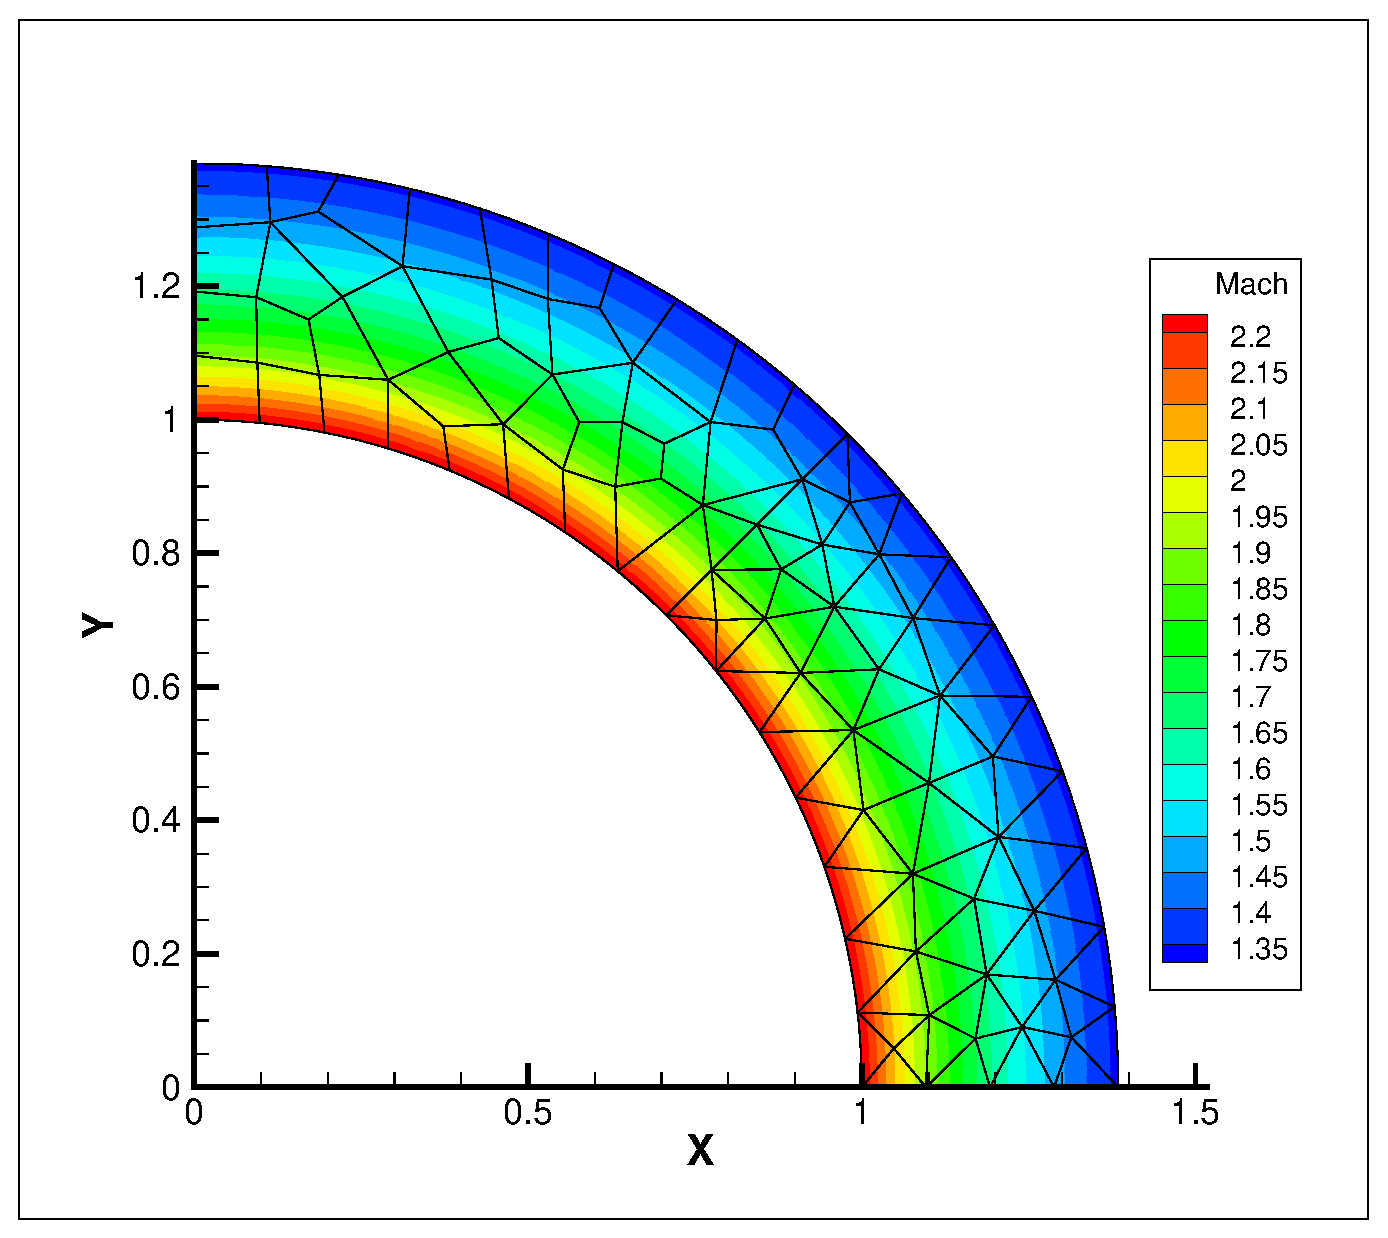
\includegraphics[width=0.8\textwidth]{./figures/SupersonicVortexMachDist_ML1P4.eps}
\caption{Mach Number Distribution: $P=4$, $PG=4$, $PF=5$, $PFr=8$, $PIs =8$, $PIc =11$, $PIsf =8$, $PIcf =12$, $EFE = 1$}
\label{fig:MachDistP4PG4PF5PFr8PIs8PIc11PIsf8PIcf12EFE1}
\end{figure}



%%%%%%%%%%%%%%%%%%%%%%%%%%%%%%%%%%%%%%%%%%%%%%%%%%%%%%%%%%%%%%%%%%
\chapter{Governing Equations}

%%%%%%%%%%%%%%%%%%%%%%%%%%%%%%%%%%%%%%%%%%%%%%%%%%%%%%%%%%%%%%%%%%
\section{Thermodynamics}

%%%%%%%%%%%%%%%%%%%%%%%%%%%%%%%%%%%%%%%%%%%%%%%%%%%%%%%%%%%%%%%%%%
\section{Navier-Stokes Equations}

%%%%%%%%%%%%%%%%%%%%%%%%%%%%%%%%%%%%%%%%%%%%%%%%%%%%%%%%%%%%%%%%%%
\section{Boundary Conditions}

%%%%%%%%%%%%%%%%%%%%%%%%%%%%%%%%%%%%%%%%%%%%%%%%%%%%%%%%%%%%%%%%%%
\section{Non-Dimensionalization}
{\color{red}Under Consideration}



%%%%%%%%%%%%%%%%%%%%%%%%%%%%%%%%%%%%%%%%%%%%%%%%%%%%%%%%%%%%%%%%%%
\chapter{Numerical Methods}
{\color{red} don't forget to add notation}
% Note about vectors being lower case and matrices upper case
% Note about multidimensional rst coordinates being written as R.
% \hat for coeffcients, \tilde for reference space.

The fundamental underlying numerical methods used for this work are presented below using a general first order PDE as a model. Emphasis is placed on the discrete representations for ease of transition between the mathematical and computational frameworks.

{\color{red} Add appendix on basis functions and derivatives.}

%%%%%%%%%%%%%%%%%%%%%%%%%%%%%%%%%%%%%%%%%%%%%%%%%%%%%%%%%%%%%%%%%%
\section{Discontinuous Petrov-Galerkin Method}

Consider the scalar 3D homogeneous conservation law,

\begin{align*}
& \frac{\partial}{\partial t} u(\vect{x},t) + \nabla \cdot \vect{f}(u(\vect{x},t)) = 0,
\hspace{2mm} t \ge 0, \hspace{2mm}
\vect{x} \coloneqq \begin{bmatrix} x & y & z \end{bmatrix} \in \Omega, \\
& u(\vect{x},0) = u_0(\vect{x}), \vect{x} \in \Omega,
\end{align*}

where $\vect{f}(u(\vect{x},t)) \coloneqq \begin{bmatrix} f_1(u(\vect{x},t)) & f_2(u(\vect{x},t)) & f_3(u(\vect{x},t)) \end{bmatrix} $ represents the fluxes in the $x$, $y$ and $z$ directions. Note that row vector notation is used throughout. The finite dimensional computational space, denoted by $\Omega^h$, is divided into $M$ elements where

\begin{equation*}
\Omega \simeq \Omega^h \coloneqq \bigcup_{m = 1}^{M} \Omega^h_m.
\end{equation*}

The global solution, $u(\vect{x},t)$, is assumed to be represented by $u^h(\vect{x},t)$, which is composed of piecewise polynomial approximations, 

\begin{equation} \nonumber
u(\vect{x},t) \simeq u^h(\vect{x},t) = \bigoplus_{m = 1}^M u^h_m(\vect{x},t).
\end{equation}

On each element, the solution is represented by a combination of $N_{vn_S}$ linearly independent modal (hierachical) or nodal (interpolating) polynomial basis functions, $\vect{\phi_{m}}(\vect{x})$, of maximal order $P$, and is generally expressed as

\begin{equation} \nonumber
\vect{x} \in \Omega_m: u^h_{m}(\vect{x},t)
=
\sum_{i=1}^{N_{vn_S}} \phi_{m,i}(\vect{x}) \hat{u}_{m,i}(t)
\coloneqq
\vect{\phi_m}(\vect{x}) \vect{\hat{u}_m}(t)^T.
\end{equation}

For tensor-product (TP), simplex (SI) and pyramidal (PYR) formulations, $N_{vn_S} = (P+1)^d$, $\frac{(P+d)!}{d!P!}$ and $\frac{(P+2)!(2P+3)}{d!P!}$, respectively, where $d$ indicates the problem dimension; wedge (WEDGE) formulations employ a combination of 2D SI and 1D TP basis functions. The elementwise residuals are given by

\begin{equation} \label{eq:residual_m}
R_m^h(\vect{x},t) 
= \frac{\partial}{\partial t} u_m^h(\vect{x},t) + \nabla \cdot \vect{f}(u_m^h(\vect{x},t))
\end{equation}

for all $M$ elements. The residuals are required to be orthogonal to a set of polynomial test functions, $\vect{\psi_{m}}(\vect{x})$, which need not be the same as the basis functions. After integration by parts, the integral weak form of the DPG scheme is obtained,

\begin{align*}
\int_{\Omega_m} \vect{\psi_m}(\vect{x})^T & \frac{\partial}{\partial t} u_m^h(\vect{x},t) -
\nabla \vect{\psi_m}(\vect{x})^T \cdot \boldsymbol f(u_m^h(\vect{x},t)) d \Omega_m \\
& + \int_{\Gamma_m} \vect{\psi_m}(\vect{x})^T \vect{\hat{n}_m} \cdot \vect{f^*}(u^h(\vect{x},t)) d \Gamma_m = \vect{0}^T, 
\end{align*}

where $\Gamma_m$ represents the element surface, $\vect{f^*}(u^h(\vect{x},t))$ denotes the numerical flux,

\begin{equation*}
\vect{\psi_{m}}(\vect{x}) \coloneqq
\begin{bmatrix} 
\psi_{m,1}(\vect{x}) & \psi_{m,2}(\vect{x}) & \dots & \psi_{m,N_{vn_T}}(\vect{x})
\end{bmatrix}
\end{equation*}

holds the test functions for the element and

\begin{equation*}
\vect{\hat{n}_m} = 
\begin{bmatrix} 
n^x & n^y & n^z
\end{bmatrix}_m.
\end{equation*}

The transformation mapping the physical coordinates to the reference coordinates on each element is expressed as

%%%%%%%%%%%%%%%%%%%%%%%%%%%%%%%%%%%%%%%%%%%%%%%%%%%%%%%%%%%%%%%%%%
\section{Adjoint Formulation}



%%%%%%%%%%%%%%%%%%%%%%%%%%%%%%%%%%%%%%%%%%%%%%%%%%%%%%%%%%%%%%%%%%
\chapter{Computational Complexity Improvements}

%%%%%%%%%%%%%%%%%%%%%%%%%%%%%%%%%%%%%%%%%%%%%%%%%%%%%%%%%%%%%%%%%%
\section{Sum Factorization}

As discussed in~\autoref{sec:Comp_comp}, sum factorization asymptotically reduces computational complexity of tensor-product operator application from $O(N^{2d})$ to $O(N^{d+1})$ where $d$ is the dimension of the problem and $N = P+1$ where $P$ is the order of the method. This is achieved by exploiting the decomposition of multi-dimensional TP operators into their 1D components, whenever both the basis functions and interpolation/cubature nodes admit such a decomposition. 

%%%%%%%%%%%%%%%%%%%%%%%%%%%%%%%%%%%%%%%%%%%%%%%%%%%%%%%%%%%%%%%%%%
\subsection{Representative Example}
The algorithm is most generally illustrated with a 3D example. Consider the case of numerical integration of the first component of the flux divergence with respect to the DG test functions as in {\color{red} refer to equation},

\begin{equation} \nonumber
\vect{\phi_r}(\mat{R_{v_I}})^T \mat{W_{v_I}} \vect{\phi}(\mat{R_{v_I}}) \vect{\hat{\tilde{f_1}}}^T
\coloneqq
\mat{D^{w}_r} \vect{\hat{\tilde{f_1}}}^T.
\end{equation}

The possibility of separation of the $\mat{D^{w}_r}$ operator into its 1D components is most easily seen by expanding the matrix operations into summations. Using indices of $b$, $t$ and $c$ to represent basis functions, test functions, and cubature nodes respectively, and visualizing $\vect{\hat{\tilde{f_1}}}$ as a 3D array with $b_1 \times b_2 \times b_3$ components,

\begin{align} \label{eq:sf_summation}
& \phi_{{t_1,t_2,t_3}_r}(\mat{R_{v_I}}) \mat{W_{v_I}} \vect{\phi}(\mat{R_{v_I}}) \vect{\hat{\tilde{f_1}}}^T \nonumber \\
= &
\sum\limits_{c_1} \sum\limits_{c_2} \sum\limits_{c_3} 
\phi_{{t_1,t_2,t_3}_r}(r_{c_1},s_{c_2},t_{c_3})
w_{c_1} w_{c_2} w_{c_3}
\vect{\phi}(r_{c_1},s_{c_2},t_{c_3}) \vect{\hat{\tilde{f_1}}}^T \nonumber \\
= &
\sum\limits_{c_1} \sum\limits_{c_2} \sum\limits_{c_3}
\phi^{1D}_{{t_1}_r}(r_{c_1}) \phi^{1D}_{t_2}(r_{c_2}) \phi^{1D}_{t_3}(r_{c_3})
w_{c_1} w_{c_2} w_{c_3}
\sum\limits_{b_1} \sum\limits_{b_2} \sum\limits_{b_3}
\phi^{1D}_{b_1}(r_{c_1}) \phi^{1D}_{b_2}(r_{c_2}) \phi^{1D}_{b_3}(r_{c_3})
\hat{\tilde{f}}_{1_{b_1,b_2,b_3}} \nonumber \\
= &
\sum\limits_{c_3} \sum\limits_{b_3} \phi^{1D}_{t_3}(r_{c_3}) w_{c_3} \phi^{1D}_{b_3}(r_{c_3})
\sum\limits_{c_2} \sum\limits_{b_2} \phi^{1D}_{t_2}(r_{c_2}) w_{c_2} \phi^{1D}_{b_2}(r_{c_2}) 
\sum\limits_{c_1} \sum\limits_{b_1} \phi^{1D}_{{t_1}_r}(r_{c_1}) w_{c_1} \phi^{1D}_{b_1}(r_{c_1})
\hat{\tilde{f}}_{1_{b_1,b_2,b_3}},
\end{align}

where summations are over the full range of each index. Assuming that the flux in reference space and test functions both use a $P_1$ basis, $\vect{\phi_r}(\vect{R})$, and using $P_2$ cubature nodes, $\mat{R_{v_I}}$, the 1D interpolation and differentiation operators can be defined as

\begin{align*}
\mat{I^{w,1D}}
\coloneqq & \hspace{1mm}
\vect{\phi^{1D}}(\vect{r_{v_I}})^T \mat{W_{vI}^{1D}} \vect{\phi^{1D}}(\vect{r_{v_I}}) \\
= &
\begin{bmatrix}
\phi^{1D}_0(r_{v_I,0}) & \phi^{1D}_0(r_{v_I,1}) & \phi^{1D}_0(r_{v_I,2}) \\
\phi^{1D}_1(r_{v_I,0}) & \phi^{1D}_1(r_{v_I,1}) & \phi^{1D}_1(r_{v_I,2}) \\
\end{bmatrix}
\begin{bmatrix}
w^{1D}_0 & 0 & 0 \\
0 & w^{1D}_1 & 0 \\
0 & 0 & w^{1D}_2 \\
\end{bmatrix}
\begin{bmatrix}
\phi^{1D}_0(r_{v_I,0}) & \phi^{1D}_1(r_{v_I,0}) \\
\phi^{1D}_0(r_{v_I,1}) & \phi^{1D}_1(r_{v_I,1}) \\
\phi^{1D}_0(r_{v_I,2}) & \phi^{1D}_1(r_{v_I,2}) \\
\end{bmatrix}
\end{align*}

and

\begin{align*}
\mat{D^{w,1D}}
\coloneqq & \hspace{1mm}
\vect{\phi^{1D}_r}(\vect{r_{v_I}})^T \mat{W_{vI}^{1D}} \vect{\phi^{1D}}(\vect{r_{v_I}}) \\
= &
\begin{bmatrix}
\phi^{1D}_{r,0}(r_{v_I,0}) & \phi^{1D}_{r,0}(r_{v_I,1}) & \phi^{1D}_{r,0}(r_{v_I,2}) \\
\phi^{1D}_{r,1}(r_{v_I,0}) & \phi^{1D}_{r,1}(r_{v_I,1}) & \phi^{1D}_{r,1}(r_{v_I,2}) \\
\end{bmatrix}
\begin{bmatrix}
w^{1D}_0 & 0 & 0 \\
0 & w^{1D}_1 & 0 \\
0 & 0 & w^{1D}_2 \\
\end{bmatrix}
\begin{bmatrix}
\phi^{1D}_0(r_{v_I,0}) & \phi^{1D}_1(r_{v_I,0}) \\
\phi^{1D}_0(r_{v_I,1}) & \phi^{1D}_1(r_{v_I,1}) \\
\phi^{1D}_0(r_{v_I,2}) & \phi^{1D}_1(r_{v_I,2}) \\
\end{bmatrix}.
\end{align*}

The standard operation can then be decomposed as

\begin{align*}
\mat{D^{w}_r} \vect{\hat{\tilde{f_1}}}^T
\coloneqq &
\begin{bmatrix}
i_{00} & 0 & 0 & 0 & i_{01} & 0 & 0 & 0 \\
0 & i_{00} & 0 & 0 & 0 & i_{01} & 0 & 0 \\
0 & 0 & i_{00} & 0 & 0 & 0 & i_{01} & 0 \\
0 & 0 & 0 & i_{00} & 0 & 0 & 0 & i_{01} \\
i_{10} & 0 & 0 & 0 & i_{11} & 0 & 0 & 0 \\
0 & i_{10} & 0 & 0 & 0 & i_{11} & 0 & 0 \\
0 & 0 & i_{10} & 0 & 0 & 0 & i_{11} & 0 \\
0 & 0 & 0 & i_{10} & 0 & 0 & 0 & i_{11} \\
\end{bmatrix}
\begin{bmatrix}
i_{00} & 0 & i_{01} & 0 & 0 & 0 & 0 & 0 \\
0 & i_{00} & 0 & i_{01} & 0 & 0 & 0 & 0 \\
i_{10} & 0 & i_{11} & 0 & 0 & 0 & 0 & 0 \\
0 & i_{10} & 0 & i_{11} & 0 & 0 & 0 & 0 \\
0 & 0 & 0 & 0 & i_{00} & 0 & i_{01} & 0 \\
0 & 0 & 0 & 0 & 0 & i_{00} & 0 & i_{01} \\
0 & 0 & 0 & 0 & i_{10} & 0 & i_{11} & 0 \\
0 & 0 & 0 & 0 & 0 & i_{10} & 0 & i_{11} \\
\end{bmatrix} \\
&
\begin{bmatrix}
d_{00} & d_{01} & 0 & 0 & 0 & 0 & 0 & 0 \\
d_{10} & d_{11} & 0 & 0 & 0 & 0 & 0 & 0 \\
0 & 0 & d_{00} & d_{01} & 0 & 0 & 0 & 0 \\
0 & 0 & d_{10} & d_{11} & 0 & 0 & 0 & 0 \\
0 & 0 & 0 & 0 & d_{00} & d_{01} & 0 & 0 \\
0 & 0 & 0 & 0 & d_{10} & d_{11} & 0 & 0 \\
0 & 0 & 0 & 0 & 0 & 0 & d_{00} & d_{01} \\
0 & 0 & 0 & 0 & 0 & 0 & d_{10} & d_{11} \\
\end{bmatrix}
\begin{bmatrix}
\hat{\tilde{f}}_{1,000} \\
\hat{\tilde{f}}_{1,100} \\
\hat{\tilde{f}}_{1,010} \\
\hat{\tilde{f}}_{1,110} \\
\hat{\tilde{f}}_{1,001} \\
\hat{\tilde{f}}_{1,101} \\
\hat{\tilde{f}}_{1,011} \\
\hat{\tilde{f}}_{1,111} \\
\end{bmatrix}.
\end{align*}

Noting that the non-zero elements in the decomposed components of $\mat{D^{w}_r}$ are built from repetition of the 1D operators and assuming that $\vect{\hat{\tilde{f}}_{1}}$ is stored continuously in memory based on sequential variation of indices $r$, $s$, then $t$, the application of the standard operator can be performed in the following steps:

\begin{enumerate}
\item Multiplication in the $r$ direction by $\mat{D^{w,1D}}$, interpreting $\vect{\hat{\tilde{f}}_{1}}$ as a $N \times N^2$ column-major matrix,

\begin{equation} \nonumber
\vect{\hat{\tilde{f}}_{1}}^{Int_1}
=
\begin{bmatrix}
d_{00} & d_{01} \\
d_{10} & d_{11} \\
\end{bmatrix}
\begin{bmatrix}
\hat{\tilde{f}}_{1,000} & \hat{\tilde{f}}_{1,010} & \hat{\tilde{f}}_{1,001} & \hat{\tilde{f}}_{1,011} \\
\hat{\tilde{f}}_{1,100} & \hat{\tilde{f}}_{1,110} & \hat{\tilde{f}}_{1,101} & \hat{\tilde{f}}_{1,111} \\
\end{bmatrix}
\end{equation}

\item Transposition of $\vect{\hat{\tilde{f}}_{1}}$, interpreted as a $N \times N^2$ column-major matrix, followed by multiplication by $\mat{I^{w,1D}}$ (in the $s$ direction), followed by a transpose interpreting the result as a $N^2 \times N$ matrix,

\begin{equation} \nonumber
\vect{\hat{\tilde{f}}_{1}}^{Int_1}
=
\begin{bmatrix}
\hat{\tilde{f}}^{Int_1}_{1,000} & \hat{\tilde{f}}^{Int_1}_{1,010} & \hat{\tilde{f}}^{Int_1}_{1,001} & \hat{\tilde{f}}^{Int_1}_{1,011} \\
\hat{\tilde{f}}^{Int_1}_{1,100} & \hat{\tilde{f}}^{Int_1}_{1,110} & \hat{\tilde{f}}^{Int_1}_{1,101} & \hat{\tilde{f}}^{Int_1}_{1,111} \\
\end{bmatrix}
\rightarrow
\begin{bmatrix}
\hat{\tilde{f}}^{Int_1}_{1,000} & \hat{\tilde{f}}^{Int_1}_{1,001} & \hat{\tilde{f}}^{Int_1}_{1,100} & \hat{\tilde{f}}^{Int_1}_{1,101} \\
\hat{\tilde{f}}^{Int_1}_{1,010} & \hat{\tilde{f}}^{Int_1}_{1,011} & \hat{\tilde{f}}^{Int_1}_{1,110} & \hat{\tilde{f}}^{Int_1}_{1,111} \\
\end{bmatrix}
\end{equation}
\begin{equation} \nonumber
\vect{\hat{\tilde{f}}_{1}}^{Int_2}
=
\begin{bmatrix}
i_{00} & i_{01} \\
i_{10} & i_{11} \\
\end{bmatrix}
\begin{bmatrix}
\hat{\tilde{f}}^{Int_1}_{1,000} & \hat{\tilde{f}}^{Int_1}_{1,001} & \hat{\tilde{f}}^{Int_1}_{1,100} & \hat{\tilde{f}}^{Int_1}_{1,101} \\
\hat{\tilde{f}}^{Int_1}_{1,010} & \hat{\tilde{f}}^{Int_1}_{1,011} & \hat{\tilde{f}}^{Int_1}_{1,110} & \hat{\tilde{f}}^{Int_1}_{1,111} \\
\end{bmatrix}
\end{equation}
\begin{equation} \nonumber
\vect{\hat{\tilde{f}}_{1}}^{Int_2}
=
\begin{bmatrix}
\hat{\tilde{f}}^{Int_1}_{1,000} & \hat{\tilde{f}}^{Int_1}_{1,001} & \hat{\tilde{f}}^{Int_1}_{1,100} & \hat{\tilde{f}}^{Int_1}_{1,101} \\
\hat{\tilde{f}}^{Int_1}_{1,010} & \hat{\tilde{f}}^{Int_1}_{1,011} & \hat{\tilde{f}}^{Int_1}_{1,110} & \hat{\tilde{f}}^{Int_1}_{1,111} \\
\end{bmatrix}
\rightarrow
\begin{bmatrix}
\hat{\tilde{f}}^{Int_2}_{1,000} & \hat{\tilde{f}}^{Int_2}_{1,010} & \hat{\tilde{f}}^{Int_2}_{1,001} & \hat{\tilde{f}}^{Int_2}_{1,011} \\
\hat{\tilde{f}}^{Int_2}_{1,100} & \hat{\tilde{f}}^{Int_2}_{1,110} & \hat{\tilde{f}}^{Int_2}_{1,101} & \hat{\tilde{f}}^{Int_2}_{1,111} \\
\end{bmatrix}
\end{equation}

\item Transposition of $\vect{\hat{\tilde{f}}_{1}}^{Int_2}$, interpreted as a $N^2 \times N$ column-major matrix, followed by multiplication by $\mat{I^{w,1D}}$ (now in the $t$ direction), followed by a transpose interpreting the result as a $N \times N^2$ matrix,
\begin{equation} \nonumber
\vect{\hat{\tilde{f}}_{1}}^{Int_2}
=
\begin{bmatrix}
\hat{\tilde{f}}^{Int_2}_{1,000} & \hat{\tilde{f}}^{Int_2}_{1,010} & \hat{\tilde{f}}^{Int_2}_{1,001} & \hat{\tilde{f}}^{Int_2}_{1,011} \\
\hat{\tilde{f}}^{Int_2}_{1,100} & \hat{\tilde{f}}^{Int_2}_{1,110} & \hat{\tilde{f}}^{Int_2}_{1,101} & \hat{\tilde{f}}^{Int_2}_{1,111} \\
\end{bmatrix}
\rightarrow
\begin{bmatrix}
\hat{\tilde{f}}^{Int_2}_{1,000} & \hat{\tilde{f}}^{Int_2}_{1,100} & \hat{\tilde{f}}^{Int_2}_{1,010} & \hat{\tilde{f}}^{Int_2}_{1,110} \\
\hat{\tilde{f}}^{Int_2}_{1,001} & \hat{\tilde{f}}^{Int_2}_{1,101} & \hat{\tilde{f}}^{Int_2}_{1,011} & \hat{\tilde{f}}^{Int_2}_{1,111} \\
\end{bmatrix}
\end{equation}
\begin{equation} \nonumber
\vect{\hat{\tilde{f}}_{1}}^{fin}
=
\begin{bmatrix}
i_{00} & i_{01} \\
i_{10} & i_{11} \\
\end{bmatrix}
\begin{bmatrix}
\hat{\tilde{f}}^{Int_2}_{1,000} & \hat{\tilde{f}}^{Int_2}_{1,100} & \hat{\tilde{f}}^{Int_2}_{1,010} & \hat{\tilde{f}}^{Int_2}_{1,110} \\
\hat{\tilde{f}}^{Int_2}_{1,001} & \hat{\tilde{f}}^{Int_2}_{1,101} & \hat{\tilde{f}}^{Int_2}_{1,011} & \hat{\tilde{f}}^{Int_2}_{1,111} \\
\end{bmatrix}
\end{equation}
\begin{equation} \nonumber
\begin{split}
\vect{\hat{\tilde{f}}_{1}}^{fin}
= &
\begin{bmatrix}
\hat{\tilde{f}}^{fin}_{1,000} & \hat{\tilde{f}}^{fin}_{1,100} & \hat{\tilde{f}}^{fin}_{1,010} & \hat{\tilde{f}}^{fin}_{1,110} \\
\hat{\tilde{f}}^{fin}_{1,001} & \hat{\tilde{f}}^{fin}_{1,101} & \hat{\tilde{f}}^{fin}_{1,011} & \hat{\tilde{f}}^{fin}_{1,111} \\
\end{bmatrix}
\rightarrow
\begin{bmatrix}
\hat{\tilde{f}}^{fin}_{1,000} & \hat{\tilde{f}}^{fin}_{1,010} & \hat{\tilde{f}}^{fin}_{1,001} & \hat{\tilde{f}}^{fin}_{1,011} \\
\hat{\tilde{f}}^{fin}_{1,100} & \hat{\tilde{f}}^{fin}_{1,110} & \hat{\tilde{f}}^{fin}_{1,101} & \hat{\tilde{f}}^{fin}_{1,111} \\
\end{bmatrix}.
\end{split}
\end{equation}
\end{enumerate}

Note that the redundant double transpose between applications of $s$ and $t$ operators can be combined into one but was not done in the interest of clarity. In the 2D TP case, the steps relating to the $t$ direction are skipped and in the 3D case using WEDGE elements, the TRI operator is interpreted as the $r$ operator, with no operator in the $s$ direction, followed by the 1D TP operation in the $t$ direction. Counting operations using general dimensions of $N$ in each coordinate direction, it is clear for the application of the fully dense standard operator that the operation count is

\begin{equation}
N^3 \times (2N^3-1) = O(N^6) = O(N^{2d}),
\end{equation}

while for the three 1D TP operators, omitting the cost of the transposes, the operation count is

\begin{equation}
3 \times N \times (2N-1) \times N^2 = O(N^4) = O(N^{d+1}).
\end{equation}

As this result is asymptotic, the advantages of the sum factorized approach are not apparent at low orders. Furthermore, for collocated schemes, TP interpolation operators are identity matrices and the standard differentiation operator becomes very sparse. Using compressed sparse row (CSR) storage, application of standard operators remains competitive with sum factorized operators for all orders tested in this case.~\autoref{sec:sf_results} presents results for timing comparisons using the different formulations.

{\color{red} don't forget to discuss implicit operators}

%%%%%%%%%%%%%%%%%%%%%%%%%%%%%%%%%%%%%%%%%%%%%%%%%%%%%%%%%%%%%%%%%%
\subsection{Timing Comparisons}
\label{sec:sf_results}

{\color{red} Add results}

\section{Representation of Operators in Fourier Space}




\chapter{TESTING FOOTNOTES}
We will now work on testing footnotes.\footnote{This is the first footnote.}
And now let's add some spurious text so that we can have a second\footnote{This
is the second footnote. To test if the footnote is typeset single-spaced, 
we add meaningless text until we can see a second line.} footnote.



	




\SetAppendixName{Appendix}%
\SetAppendixText{Here is the text of an Appendix.  If only one appendix is required, place it here.}%
\ETDAppendix{Appendix A}{Here is the text of an Appendix.}%
\ETDAppendix{Appendix B}{Here is the text of a second, additional Appendix}%
%\end{\ETDAppendix}%

\bibHeading{\uppercase{References}}
\bibliography{PhD_Thesis}
\bibliographystyle{elsarticle-num}
%\bibliographystyle{plain}



\end{document}\grid
